%% abtex2-modelo-artigo.tex, v-1.9.6 laurocesar
%% Copyright 2012-2016 by abnTeX2 group at http://www.abntex.net.br/ 
%%
%% This work may be distributed and/or modified under the
%% conditions of the LaTeX Project Public License, either version 1.3
%% of this license or (at your option) any later version.
%% The latest version of this license is in
%%   http://www.latex-project.org/lppl.txt
%% and version 1.3 or later is part of all distributions of LaTeX
%% version 2005/12/01 or later.
%%
%% This work has the LPPL maintenance status `maintained'.
%% 
%% The Current Maintainer of this work is the abnTeX2 team, led
%% by Lauro César Araujo. Further information are available on 
%% http://www.abntex.net.br/
%%
%% This work consists of the files abntex2-modelo-artigo.tex and
%% abntex2-modelo-references.bib
%%

% ------------------------------------------------------------------------
% ------------------------------------------------------------------------
% abnTeX2: Modelo de Artigo Acadêmico em conformidade com
% ABNT NBR 6022:2003: Informação e documentação - Artigo em publicação 
% periódica científica impressa - Apresentação
% ------------------------------------------------------------------------
% ------------------------------------------------------------------------

\documentclass[
% -- opções da classe memoir --
article,			% indica que é um artigo acadêmico
12pt,				% tamanho da fonte
a4paper,			% tamanho do papel. 
% -- opções da classe abntex2 --
%chapter=TITLE,		% títulos de capítulos convertidos em letras maiúsculas
%section=TITLE,		% títulos de seções convertidos em letras maiúsculas
%subsection=TITLE,	% títulos de subseções convertidos em letras maiúsculas
%subsubsection=TITLE % títulos de subsubseções convertidos em letras maiúsculas
% -- opções do pacote babel --
english,			% idioma adicional para hifenização
brazil,				% o último idioma é o principal do documento
sumario=tradicional,
twoside
]{abntex2}


% ---
% PACOTES
% ---

% ---
% Pacotes fundamentais 
% ---
\usepackage{lmodern}			% Usa a fonte Latin Modern
\usepackage[T1]{fontenc}		% Selecao de codigos de fonte/ tipos.
\usepackage[utf8]{inputenc}		% Cconversão automática dos acentos - direto do teclado
%\usepackage{indentfirst}		% Indenta o primeiro parágrafo de cada seção.
\usepackage{nomencl} 			% Lista de simbolos
\usepackage{color}				% Controle das cores
\usepackage{microtype} 			% para melhorias de justificação
\usepackage{url}
% ---

% ---
% Pacotes adicionais, usados apenas no âmbito do Modelo Canônico do abnteX2
% ---
\usepackage{lipsum}				% para geração de dummy text
% ---

%----- Acrescentado por SKJr: início
\usepackage{amsthm}     % melhoria estrutura matemática
%\usepackage{NotesTeX}  % notas nas margens
\usepackage{multicol}   % mesclar colunas tabela
\usepackage{multirow}   % mesclar linhas tabela
\usepackage{textcomp}   % Text Companion fonts
\usepackage{amsmath}    % pacote matemático
\usepackage{wasysym}    % pacote de símbolos com telefone
\usepackage{ marvosym } % pacote de símbolos com e-mail
\usepackage{colortbl}   % permite tabela com cor
\usepackage{subcaption} % permite tabela de figuras

%----  Numera questoes e repostas ---
\usepackage{exsheets} 
\usepackage{tasks}
\SetupExSheets[question]{type=exam}
\SetupExSheets{
	counter-format=se.qu,
	counter-within=section,
	headings=runin,
}
%----- Acrescentado por SKJr: fim


% ---
% Pacotes de citações
% ---
\usepackage[brazilian,hyperpageref]{backref}	 % Paginas com as citações na bibl
\usepackage[alf]{abntex2cite}	% Citações padrão ABNT
% ---

% ---
% Configurações do pacote backref
% Usado sem a opção hyperpageref de backref
\renewcommand{\backrefpagesname}{Citado na(s) página(s):~}
% Texto padrão antes do número das páginas
\renewcommand{\backref}{}
% Define os textos da citação
\renewcommand*{\backrefalt}[4]{
	\ifcase #1 %
	Nenhuma citação no texto.%
	\or
	Citado na página #2.%
	\else
	Citado #1 vezes nas páginas #2.%
	\fi}%
% ---

% ---
% Informações de dados para CAPA e FOLHA DE ROSTO
% ---
\titulo{\huge\textsc{Análise de Sentimentos em comentários no Twitter}\\ \Large{}}
\autor{
	Danilo Silva Bentes
	\\
	Gabriel Augusto De Vito D'Abmauia Guimarães 
}
\local{Brasil}
\data{2018, v-1.3}
% ---

% ---
% Configurações de aparência do PDF final

% alterando o aspecto da cor azul
\definecolor{blue}{RGB}{41,5,195}
\definecolor{green}{rgb}{0.1,0.1,0.1}

% informações do PDF
\makeatletter
\hypersetup{
	%pagebackref=true,
	pdftitle={\@title}, 
	pdfauthor={\@author},
	pdfsubject={Roteiro de Laboratório},
	pdfcreator={LaTeX with abnTeX2},
	pdfkeywords={abnt}{latex}{abntex}{abntex2}{atigo científico}, 
	colorlinks=true,       		% false: boxed links; true: colored links
	linkcolor=blue,          	% color of internal links
	citecolor=blue,        		% color of links to bibliography
	filecolor=magenta,      		% color of file links
	urlcolor=blue,
	bookmarksdepth=4
}
\makeatother
% --- 

% ---
% compila o indice
% ---
\makeindex
% ---

% ---
% Altera as margens padrões
% ---
\setlrmarginsandblock{3cm}{3cm}{*}
\setulmarginsandblock{3cm}{3cm}{*}
\checkandfixthelayout
% ---

% --- 
% Espaçamentos entre linhas e parágrafos 
% --- 

% O tamanho do parágrafo é dado por:
\setlength{\parindent}{1.3cm}

% Controle do espaçamento entre um parágrafo e outro:
\setlength{\parskip}{0.2cm}  % tente também \onelineskip

% Espaçamento simples
\SingleSpacing


% Margin Figure configuration
\usepackage{graphicx}
%\usepackage[dvipsnames]{xcolor}
\usepackage{caption}[2008/04/01]
\usepackage{wrapfig} %tabulação de figuras
\captionsetup{justification=raggedright,labelfont={bf},font=small} %posição de caption


% ----
% Início do documento
% ----
\begin{document}
	
	% Seleciona o idioma do documento (conforme pacotes do babel)
	%\selectlanguage{english}
	\selectlanguage{brazil}
	
	% Retira espaço extra obsoleto entre as frases.
	\frenchspacing 
	
	% ----------------------------------------------------------
	% ELEMENTOS PRÉ-TEXTUAIS
	% ----------------------------------------------------------
	
	%---
	%
	% Se desejar escrever o artigo em duas colunas, descomente a linha abaixo
	% e a linha com o texto ``FIM DE ARTIGO EM DUAS COLUNAS''.
	% \twocolumn[    		% INICIO DE ARTIGO EM DUAS COLUNAS
	%
	%---
	% página de titulo
	\maketitle
	

	
	% ]  				% FIM DE ARTIGO EM DUAS COLUNAS
	% ---
	
	% ----------------------------------------------------------
	% ELEMENTOS TEXTUAIS
	% ----------------------------------------------------------
	\textual
	
	% ----------------------------------------------------------
	% Introdução
	% ----------------------------------------------------------
	\section{Introdução}
	A análise de sentimentos, também conhecida como mineração de opiniões, refere-se ao uso de \emph{Processamento de Linguagem Natural} para identificar, extrair, quantificar e estudar o estado afetivo e subjetivo da informação.

	Este é um recurso muito importante, principalmente para empresas que desejam saber qual é a opinião que as pessoas estão tendo sobre seus produtos lançados no mercado.
	
	A Web é um excelente meio de se extrair dados e de se retirar informações importantes, tanto por meio das redes sociais quanto por sites de notícias, blogs ou outras plataformas. É incontestável que a Web é palco de opiniões de usuários sobre produtos, críticas, elogios, comentários, etc.
	
	\section{Objetivo}
	
	Nosso objetivo com este artigo é demonstrar como o método probabilístico \emph{Naive Bayes} (explicado na seção \ref{naive}) pode ser útil para determinar a polaridade de uma frase ou comentário, tendo como aprendizado uma base de dados previamente classificada. Ou seja, determinar qual é a eficácia deste método em dizer se uma determinada frase tem cunho \textbf{positivo}, \textbf{negativo} ou \textbf{neutro} dada uma tabela de dados previamente classificada.
	
	\section{Desenvolvimento}
	
	
	
	\subsection{Base de dados}
	\label{Base}
	Necessitamos de uma base de dados classificada a fim de "treinarmos" o nosso modelo. O objetivo é que o algoritmo que desenvolvermos possa ler esta base e "aprender" qual palavra é 'positiva', 'negativa', ou 'neutra'.
	
	Utilizamos uma base de dados composta por 8199 linhas contendo comentários diversos retirados de tweets do Twitter. Esta base de dados foi retirada do sítio
	\cite{minerandodados},  e possui duas colunas principais: \emph{A frase propriamente dita} e a sua \emph{classificação}.
	
		
	\subsection{Pré-processamento}
	O pré-processamento inicia-se quando os dados são coletados e organizados na forma de um conjunto de dados. Existem diversos objetivos nesta fase e um deles é solucionar os possíveis problemas com a base com que estamos trabalhando, tais como identificar atributos irrelevantes, valores desconhecidos, possíveis caracteres em lugares errados ou que irão atrapalhar a análise do algoritmo.
	
	Nós utilizamos os seguintes recursos de pré-processamento:
	\begin{enumerate}
		\item Tokenização: É utilizada em decompor cada o documento em cada termo que o compõe. Utilizamos espaços em branco para separar palavra por palavra de cada frase existente no documento.
		\item Limpeza: Foram removidas as vírgulas, aspas, dois pontos, arrobas e outros símbolos que estavam sujando a análise. Portanto, deixamos, para cada token, apenas palavras que contenham letras de A-Z, a-z, acentuações básicas e números.
		Devemos lembrar que a nossa base de dados é composta por tweets e a tokenização separando as palavras por espaços em branco podem causar problemas. Por exemplo: a palavra 'amor' é diferente de 'amor:' ou '@amor'. Portanto, a limpeza é fundamental para o bom funcionamento do método.
	\end{enumerate}
	
	Observação: A \emph{remoção de stopwords} é um recurso muito utilizado no 
	pré-processamento de dados. Porém, não o utilizamos, pois afetaria de forma negativa os nossos resultados. Há frases em que remover as stopwords faria com que a sua polaridade mudasse completamente. Um exemplo seria: "Eu não gostei deste governante, não votaria nele novamente" (negativa). Após removermos a stopword "não", a frase tornaria-se positiva.
	
	
	\label{naive}
	\subsection{Naive Bayes}
	Utilizaremos o algoritmo \emph{Naive Bayes}, que supõe que exista uma independência entre as palavras (features) do modelo. 
	
	Trata-se de um modelo puramente probabilístico, e não se baseia de redes neurais artificiais para fazer predições.
	
	O algoritmo recebe o nome de ingênuo (naive), pois para se classificar uma sentença como positiva, negativa ou neutra, ele faz a classificação palavra por palavra.
	
	 Caso o número de palavras classificadas como positiva dentro de uma sentença seja maior do que o número de palavras classificadas como negativa, então essa sentença é considerada positiva. Do contrário, se a frase possui mais palavras negativas do que positivas, ela é considerada uma frase negativa. Caso o número de palavras positivas seja igual ao número de palavras negativas, então essa frase é taxada como neutra.
	
	
	\textbf{Um exemplo mais concreto de como o algoritmo funciona}
	
	Utilizando um exemplo simples, podemos mostrar, passo-a-passo, como funciona o algoritmo \emph{Naive Bayes}:
	
	% ----------------------------------------------------------
	% EXEMPLO DE BASE DE DADOS
	% ----------------------------------------------------------
	A partir de uma base de dados, como a que temos no nosso projeto, suponha que exista um trecho desta base com as seguintes classificações:
	
	\begin{table}[!h]
		\caption{Exemplo fictício de uma base de dados com a classificação de cada palavra}
		\label{tab: baseDados1}
		\centering
		
		\begin{tabular}{|c|c|} \hline
			\textbf{Palavra} & \textbf{Classe} \\
			\hline
		
			cachorro	& positivo \\
			amor &	negativo \\
			mau	& negativo \\
			amor & positivo \\
			amor &	positivo \\
			cachorro	& positivo \\
			casa &	positivo \\
			gato	& positivo \\
			gato	& negativo \\
			gato	& negativo \\
			amor & 	negativo \\
			casa	& positivo \\
			amor	& positivo \\
			
			\hline
			
		\end{tabular}
			
	\end{table}

	
	% ----------------------------------------------------------
	% TABELA DE FREQUÊNCIA
	% ----------------------------------------------------------
	Agora que temos uma base de dados classificada, o próximo passo é criarmos uma tabela de frequência, mostrando, para cada palavra, quantas vezes ela apareceu como positiva ou negativa nessa base de dados.
	
	\begin{table}[h]
		\caption{Tabela de frequência}
		\label{tab: tabelaFrequencia}
		\centering
		
		\begin{tabular}{|c|c|c|} \hline
			\textbf{Palavra} & \textbf{Positivo} & \textbf{Negativo} \\
			\hline
			cachorro	& 2 & 0 \\
			amor & 3 & 2 \\
			mau & 0 & 1 \\
			gato & 1 & 3 \\
			casa & 2 & 0 \\
			\hline
			Total & 8 & 6 \\
			\hline
			
		\end{tabular}
		
	\end{table}
	
	% ----------------------------------------------------------
	% TABELA DE PROBABILIDADES
	% ----------------------------------------------------------
	Tendo em mãos a tabela de frequência, podemos criar uma tabela de probabilidades para, então, podermos calcular qual é a probabilidade de uma determinada palavra ser \emph{positiva} ou \emph{negativa} no nosso 'treino'.
	
	\begin{table}[!h]
		\caption{Tabela de Probabilidades}
		\label{tab: tabelaProbabilidades}
		\centering
		
		\begin{tabular}{|c|c|c|c|} \hline
			\textbf{Palavra} & \textbf{Positivo} & \textbf{Negativo} & \textbf{Frequência} \\
			\hline
			cachorro	& 2 & 0 & $\frac{2}{14} = 0.142$ \\
			amor & 3 & 2 & $\frac{5}{14} = 0.357$ \\
			mau & 0 & 1 & $\frac{1}{14} = 0.071$ \\
			gato & 1 & 3 & $\frac{4}{14} = 0.285$ \\
			casa & 2 & 0 & $\frac{2}{14} = 0.142$ \\
			\hline
			Total & 8 & 6 & \\
			\hline
			& $\frac{8}{14} = 0.571$ & $\frac{6}{14} = 0.428 $ & \\
 			\hline
		\end{tabular}
		
	\end{table}

	O algoritmo de Naive Bayes consegue calcular a probabilidade de cada palavra ser positiva ou negativa seguindo o seguinte exemplo:
	
	\begin{eqnarray}
		\label{eq: equacaoNaiveBayes}
		P(positivo|'amor') = \frac{P('amor'|positivo) * P(positivo)}{P('amor')} \\
		P(negativo|'amor') = \frac{P('amor'|negativo) * P(negativo)}{P('amor')} 
	\end{eqnarray}
	
	Realizando os cálculos necessários para computar a probabilidade da palavra 'amor' ser positiva e negativa, temos:
	\begin{eqnarray}
		P('amor') = \frac{5}{14} = 0.357 \\
		P('amor'|positivo) = \frac{3}{8} = 0.375 \\
		P('amor'|negativo) = \frac{2}{6} = 0.33\\
		P(positivo) = \frac{8}{14} = 0.571 \\
		P(negativo) = \frac{6}{14} = 0.428 \\
		P(positivo|'amor') = \frac{0.375 * 0.571}{0.357} = \textbf{0.599}\\
		P(negativo|'amor') = \frac{0.33 * 0.428}{0.357} = \textbf{0.395} 
	\end{eqnarray}
	
	Facilmente percebemos que a probabilidade da palavra 'amor' ser positiva é maior do que a probabilidade dela ser negativa. 
	
	Portanto, sempre que a palavra 'amor' aparecer em uma frase de teste, devemos contabilizá-la como positiva dentro desta frase.
	
	Fazendo esta classificação com todas as palavras deste exemplo, temos uma outra tabela, denominada \emph{tabela de classificação}, contendo a palavra e a classificação (label) que o algoritmo determinou para cada palavra.
	
	\begin{table}[!h]
		\caption{Tabela de Classificação}
		\label{tab: labels}
		\centering
		
		\begin{tabular}{|c|c|} \hline
			\textbf{Palavra} & \textbf{Classificação} \\
			\hline
			cachorro & Positivo \\
			amor & Positivo \\
			mau & Negativo \\
			casa & Positivo \\
			gato & Negativo \\
			\hline
		\end{tabular}
		
	\end{table}
	
	\subsection{Teste do algoritmo}
	Tendo em mãos a tabela \ref{tab: labels}, podemos começar um exemplo de teste. 
	O teste consiste em frases contendo palavras conhecidas na classificação ou não.
	Percorremos essas frases e, para cada frase, contabilizamos quantas palavras desta frase são positivas, negativas e neutras. 
	
	Caso o número de palavras positivas seja superior ao número de palavras negativas e neutras, então essa frase é classificada como positiva. A mesma regra é utilizada para frases que possuem maior número de palavras negativas ou neutras.
	
	Caso a frase contenha uma ou mais palavras \emph{desconhecidas}, elas serão descartadas na contagem. Este é um problema do algoritmo e está citado na seção \ref{melhorias} (melhorias a serem feitas), pois se uma frase contém 80\% das palavras desconhecidas, não é justo classificá-la baseada em 20\% das palavras que a compõe.
	
	Caso nenhuma palavra da frase possua classificação, então essa frase receberá a classificação de maior frequência no treino.
	
	\section{O algoritmo desenvolvido}
	
	\subsection{Treino}
	
	Com posse de nossa base de dados citada em \ref{Base}, desenvolvemos um algoritmo em Python, que percorre as 7000 primeiras frases desta base e, para cada frase, monta a tabela de frequência igual à tabela \ref{tab: tabelaFrequencia}, a armazena na memória e calcula a probabilidade de cada palavra ser positiva, negativa ou neutra, baseando-se na equação \ref{eq: equacaoNaiveBayes}, tendo como resultado uma tabela semelhante à tabela \ref{tab: labels}, porém com a classificação de cada palavra da base.
	
	Utilizamos apenas 7000 frases, e não todas, para forçarmos que nosso teste tenha algumas palavras desconhecidas, a fim de fazermos com que nosso modelo se aproxime mais de um modelo real.
	
	Ao executarmos o nosso algoritmo, vimos que a nossa tabela \ref{tab: labels} tem 
	
	Desta maneira, o algoritmo passa a ter posse de 115111 palavras classificadas, das quais 26.84\% foram classificadas como positivas, 37.67\% como negativas e 35,49\% neutras.
	O tempo de execução foi 10.46 segundos. A imagem \ref{fig: treino} mostra a etapa de treino sendo executada em um processador core i5.
	
	\begin{figure}[h!]
		\centering
		\caption{Execução da parte de treino do algoritmo}
		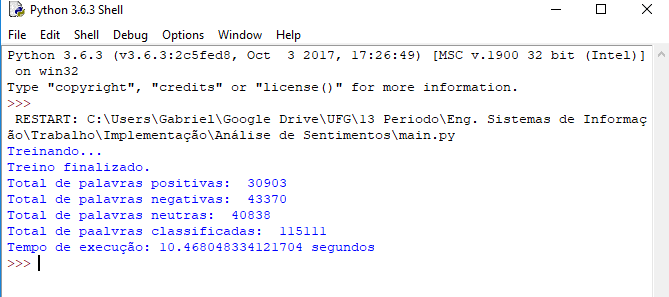
\includegraphics[scale=1]{treino.png}
		\fonte{Próprio autor}
		\label{fig: treino}
	\end{figure}
	
	Não utilizamos toda a base de dados para treinar a classificação pois desejamos que algumas palavras no teste sejam desconhecidas, para dar um comportamento mais realista para o nosso modelo.
	
	\subsection{Teste}
	
	\label{teste}
	O teste é a parte mais importante do algoritmo. Buscamos, dentro desta mesma base de dados, 1700 frases \textbf{aleatórias} para testarmos. Devido ao caráter aleatório das frases, a cada instância de execução do teste teremos resultados distintos. Portanto, faremos uma média de execução.
	
	O teste consiste em:
	\begin{enumerate}
		\item Carregar as frases de teste na memória.
		\item Para cada palavra de cada frase do teste, verificar a classificação desta palavra na instância de treino (na tabela \ref{tab: labels}) e somar as contribuições positivas, negativas e neutras de cada palavra dentro desta frase.
		\item Caso o número de palavras positivas em uma frase seja maior do que o número de palavras negativas e neutras, então esta frase deve ser classificada como positiva. Repetir a mesma lógica para palavras negativas e neutras.
		\item Comparar a classificação do teste com a classificação da base de dados. Caso sejam iguais, então significa que o algoritmo \emph{acertou} o resultado. Caso sejam diferentes, classificar este teste como \emph{erro}.
	\end{enumerate}

		Uma consideração importante sobre o teste: caso uma palavra no teste não seja reconhecida, ou seja, ainda não tenha sido lida na fase de treino ou não está classificada, \textbf{é atribuída a ela a classificação de maior frequência}.
		
		Como citado acima, o caráter aleatório do nosso algoritmo nos força a testar mais de uma vez para termos uma média de erros e acertos. Realizamos, portanto, dez testes como o ilustrado na figura \ref{fig: teste1}. A tabela \ref{tab: testes} mostra os resultados desses testes, bem como a \textbf{média de acertos} e \textbf{média de erros}.  
		
		\begin{figure}[h!]
			\centering
			\caption{Execução de um dos testes}
			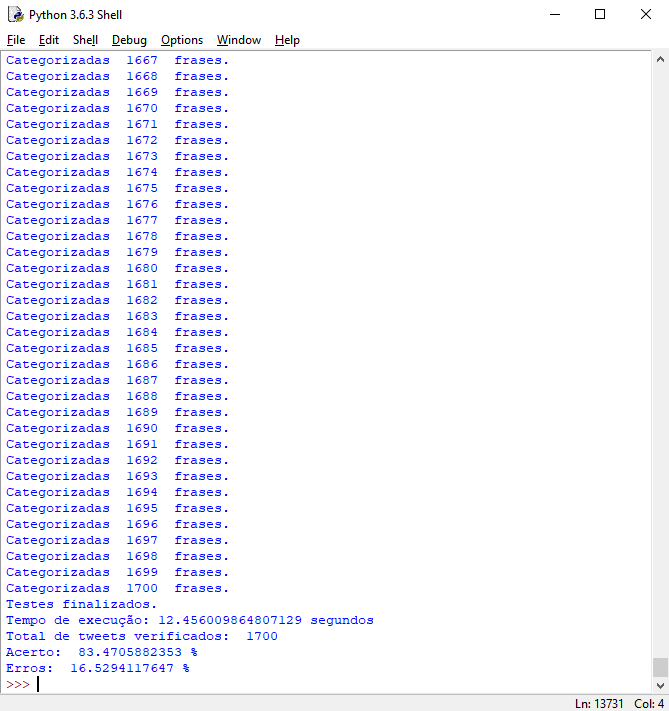
\includegraphics[scale=1]{teste1.png}
			\fonte{Próprio autor}
			\label{fig: teste1}
		\end{figure}
	
		\begin{table}[!h]
			\caption{Resultados dos testes realizados}
			\label{tab: testes}
			\centering
			
			\begin{tabular}{|c|c|c|c|} \hline
				\textbf{Teste} & \textbf{Acertos \%} & \textbf{Erros \%} & \textbf{Tempo(s)\%} \\
				\hline
				1 & 85.00 & 15.0 & 15.82\\
				2 & 84.05 & 15.94 & 9.24 \\
				3 & 80.82 & 19.17 & 12.89 \\
				4 & 83.41 & 16.58 & 14.24\\
				5 & 82.67 & 17.23 & 13.09 \\
				6 & 83.41 & 16.58 & 12.52\\
				7 & 81.76 & 18.23 & 12.49\\
				8 & 83.76 & 16.23 & 12.48\\
				9 & 82.23 & 17.76 & 12.35\\
				10 & 83.47 & 16.53 & 12.45\\
				\hline
				Média & 83.06  &  16.92  & 12.45 \\
				\hline
				
			\end{tabular}
			
		\end{table}
		
		Notamos que o algoritmo se mostra bastante eficaz quando separadas 1700 frases aleatórias para teste, retiradas do mesmo conjunto de dados. Dessas 1700 frases, houve uma média de acerto de 83.06\%, o que corresponde a 1412 frases classificadas da maneira correta.
		
		O tempo de execução dependerá das configurações da sua CPU ou GPU, mas não é um fator limitante para essa quantidade de dados, visto que a média de 12.45 segundos não é um tempo preocupante.
		
		
	\section{Melhorias no método}
	\label{melhorias}
	\subsection{Teoria}
	Ao longo do desenvolvimento deste algoritmo e deste artigo, percebemos que poderíamos fazer algumas modificações para melhorarmos o nosso modelo e torná-lo mais real e aplicável.
	
	A primeira modificação foi adicionar um peso para cada palavra, ou seja, atribuir a ela o \emph{quanto} é positiva, negativa ou neutra, levando em consideração a frequência com que esta palavra aparece em cada uma dessas classificações. 
	
	Este "peso"  nada mais é do que a divisão da frequência com que esta palavra aparece como positiva, negativa ou neutra dividida pelo total de palavras positivas, negativas ou neutras, respectivamente. Este peso será contabilizado na instância de teste, de tal forma que cada palavra tenha uma contribuição numérica e a soma das contribuições positivas, negativas ou neutras de todas as palavras da frase irão determinar a sua classificação.
	
	
	Utilizando a tabela de frequências (\ref{tab: tabelaFrequencia}) e a equação Naive Bayes (\ref{eq: equacaoNaiveBayes}), chegamos à tabela de classificação (\ref{tab: labels}), exatamente igual ao método anterior. Porém, agora, a diferença é que temos uma tabela adicional: a tabela de pesos (\ref{tab: tabfreq2}).
 
	\begin{table}[!h]
		\caption{Tabela de frequência com o peso de cada palavra}
		\label{tab: tabfreq2}
		\centering
		
		\begin{tabular}{|c|c|c|c|c|} \hline
			\textbf{Palavra} & \textbf{Positivo} & \textbf{Negativo} & \textbf{Peso (pos)} & \textbf{Peso (neg)}\\
			\hline
			cachorro & 2 & 0 & 0.25 & 0\\
			amor & 3 & 2 & 0.38 & 0.33\\
			mau & 0 & 1 & 0 & 0.16\\
			gato & 1 & 3 & 0.13 & 0.5\\
			casa & 2 & 0 & 0.25 & 0\\
			\hline
			Total & 8 & 6  & - & - \\
			\hline
			
		\end{tabular}
	\end{table}

    Lembrando que o cálculo do peso segue a seguinte equação:
	
	\begin{equation}
	Peso = \frac{P(positiva|palavra)}{\sum(positivas)}
	\end{equation}
	
	O que percebemos com a tabela \ref{tab: tabfreq2} é que a palavra "amor"  é "mais positiva"  do que a palavra "casa", por exemplo. Apesar de ambas serem positivas, existe um peso maior na palavra "amor" e este peso será levado em consideração no treino.

	Lembrando que devemos ignorar o peso negativo e neutro da palavra, caso ela já tenha sido classificada como positiva. Ignorar o peso positivo e neutro caso ela tenha sido classificada como negativa. E ignorar os pesos positivo e negativo caso ela seja neutra.
	 
	Como exemplo, suponhamos a seguinte sentença de teste:
	\begin{quote}
		"cachorro amor mau gato amor"
	\end{quote}
    
    
	\begin{table}[!h]
		\caption{Palavra, classificação e soma dos pesos}
		\label{tab: tabfreq3}
		\centering
		
		\begin{tabular}{|c|c|c|c|} \hline
			\textbf{Palavra} & \textbf{Classificação} & \textbf{Peso (pos)} & \textbf{Peso (neg)}\\
			\hline
			cachorro & Positivo & 0.25 & -\\
			amor & Positivo & 0.38 & - \\
			mau & Negativo & - & 0.16\\
			gato & Negativo & - & 0.5\\
			amor & Positivo & 0.38 & -\\
			\hline
			Somatório & - & 1.01 & 0.66 \\
			\hline
			
		\end{tabular}
		
	\end{table}	
	
	Perceba, na tabela \ref{tab: tabfreq3}, que quando uma palavra é positiva, nós devemos levar em consideração apenas o peso positivo desta palavra. 
	
	O somatório dos pesos positivos foram maiores do que dos pesos negativos. 
	Logo, esta sentença é considerada positiva.
	
	A diferença deste método para o outro é que talvez uma palavra seja tão negativa que acabe compensando um número maior de palavras positivas com pesos menores e faça uma sentença com um grande número de palavras positivas se tornar negativa devido ao peso desta palavra.
	
	\subsection{Resultados}
	Fizemos essa modificação no nosso algoritmo e, novamente, o executamos 10 vezes.
	\begin{figure}[h!]
		\centering
		\caption{Execução da parte de treino do algoritmo melhorado}
		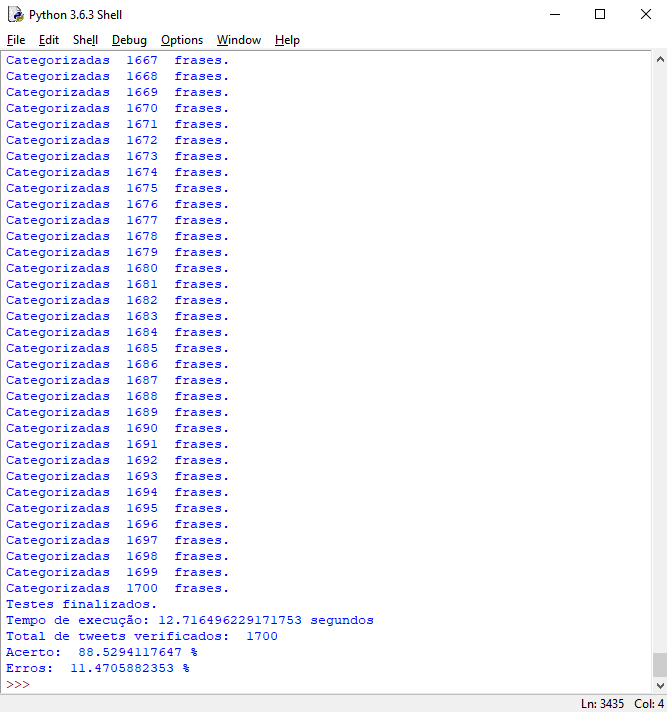
\includegraphics[scale=1]{melhoria1.png}
		\fonte{Próprio autor}
		\label{fig: melhoria1}
	\end{figure}
	
	% ----------------------------------------------------------
	% Referências bibliográficas
	% ----------------------------------------------------------
	\newpage
	\nocite{sitenaive}
	\bibliography{referencias}
	
	
\end{document}
